\begin{table*}
\centering
\renewcommand{\tabcolsep}{6pt}
\scalebox{0.62}{
\begin{tabular}{|l||rrrr|rrrr|rrrr|rrrr|rrrr|}
\multicolumn{1}{c}{} & \multicolumn{4}{c}{Middlebury 2014 (H)} & \multicolumn{4}{c}{Middlebury 2021} & \multicolumn{4}{c}{ETH3D} & \multicolumn{4}{c}{KITTI 2012} & \multicolumn{4}{c}{KITTI 2015} \\
\hline
 \multirow{2}{*}{Model} & \multicolumn{3}{c}{bad $>2$} & Avg. & \multicolumn{3}{c}{bad $>2$} & Avg. & \multicolumn{3}{c}{bad $>1$} & Avg. & \multicolumn{3}{c}{bad $>3$} & Avg. & \multicolumn{3}{c}{bad $>3$} & Avg. \\
  & All & Noc & Occ & (px) & All & Noc & Occ & (px) & All & Noc & Occ & (px) & All & Noc & Occ & (px) & All & Noc & Occ & (px) \\
\hline\hline
{RAFT-Stereo} \cite{lipson2021raft} 
& 11.15 & 8.06 & 29.06 & \trd 1.55 
& 12.05 & 9.38 & 37.89 & 1.81 
&\snd 2.59 &\snd 2.24 & \snd 8.78 &\fst 0.25 
& \trd 4.80 & \trd 3.70 & \snd 28.54 & \snd 0.89 
& \trd 5.44 & \trd 4.69 & \trd 13.52 & \snd 1.16 \\
{PSMNet} \cite{chang2018pyramid} 
& 18.79 & 13.80 & 53.22 & 4.63 
& 23.67 & 20.61 & 53.75 & 5.70 
& 19.75 & 18.62 & 42.05 & 0.94 
& 6.73 & 5.28 & 45.48 & 1.22 
& 6.78 & 5.84 & 24.22 & 1.38 \\
{GMStereo} \cite{xu2023unifying} 
& 15.63 & 10.98 & 46.04 & 1.87 
& 25.43 & 22.43 & 54.70 & 2.86 
& 6.22 & 5.58 & 19.97 & 0.42 
& 5.68 & 4.34 & 38.12 & 1.10 
& 5.72 & 4.92 & 16.74 & 1.21 \\
{ELFNet} \cite{lou2023elfnet} 
& 24.48 & 16.94 & 77.06 & 8.61 
& 27.08 & 21.77 & 85.56 & 11.01 
& 25.61 & 24.50 & 46.06 & 5.65 
& 10.52 & 8.13 & 87.24 & 2.30 
& 9.61 & 7.67 & 84.71 & 2.16 \\
{PCVNet} \cite{Zeng_2023_ICCV} 
& 18.50 & 14.73 & 42.16 & 3.45 
& 18.40 & 15.06 & 51.50 & 3.84 
& 7.81 & 7.19 & 20.07 & 0.69 
& 5.14 & 3.95 & 32.07 & 0.95 
& 5.49 & 4.74 & 15.14 & 1.34 \\
{DLNR} \cite{zhao2023high} 
& \snd 9.46 & \snd 6.20 & \trd 28.75 & \snd 1.45 
&\snd 8.44 &\snd 5.88 & \fst 32.71 & \snd 1.24 
& 23.12 & 22.94 & 26.93 & 9.89 
& 9.45 & 8.30 & 36.05 & 1.59 
& 15.74 & 14.87 & 33.65 & 2.83 \\
{Selective-RAFT} \cite{wang2024selective} 
& 12.05 & 9.46 & 27.42 & 2.35 
& 15.69 & 13.86 & 36.32 & 5.92 
& 4.36 & 3.81 & \trd 10.23 & \trd 0.34 
& 5.71 & 4.63 & \trd 29.87 & 1.08 
& 6.50 & 5.69 & 17.85 & 1.27 \\
{Selective-IGEV} \cite{wang2024selective} 
& \trd 9.98 & \trd 7.09 & \snd 27.62 & 1.60 
& \trd 8.89 & \trd 6.34 & \trd 32.88 & \trd 1.60 
& 6.42 & 5.71 & 18.71 & 1.73 
& 6.22 & 4.91 & 34.08 & 1.09 
& 5.87 & 5.15 & 14.42 & 1.42 \\
{IGEV-Stereo} \cite{xu2023iterative} 
& 15.07 & 11.81 & 35.78 & 3.20 
& 20.43 & 18.14 & 45.37 & 8.16 
& 43.05 & 42.42 & 57.19 & 1.04 
& 7.62 & 5.90 & 56.13 & 1.50 
& 7.81 & 6.68 & 42.29 & 1.56 \\
{NMRF} \cite{guan2024neural} 
& 14.08 & 10.87 & 34.62 & 2.91 
& 23.36 & 21.69 & 42.51 & 8.57 
& \trd 4.34 & \trd 3.66 & 17.15 & 0.42 
& \snd 4.62 & \snd 3.52 & 29.98 & \trd 0.92 
& \snd 5.24 & \snd 4.55 & \snd 11.72 & \snd 1.16 \\
{\bf \method{} (ours)} 
&\fst 7.07 &\fst 4.76 &\fst 20.77 &\fst 0.97
& \fst 8.38 & \fst 5.86 &\snd 32.87 &\fst 1.10 
& \fst 2.39 & \fst 2.16 &\fst 5.82 & \snd 0.28 
&\fst 3.94 &\fst 3.03 &\fst 21.02 &\fst 0.85 
&\fst 3.98 &\fst 3.29 &\fst 10.55 &\fst 0.97 \\

\hline
\end{tabular}}\vspace{-0.2cm}
\caption{\textbf{Zero-shot Generalization.} Comparison with state-of-the-art deep stereo models. Networks trained on SceneFlow \cite{mayer2016large}.
}\vspace{-0.3cm}
\label{tab:roundtable1}
\end{table*}

\begin{figure*}[t]
    \centering
    \renewcommand{\tabcolsep}{1pt}
    \begin{tabular}{ccccccc}
        & \small RGB &
        \small RAFT-Stereo \cite{lipson2021raft} &
        \small DLNR \cite{zhao2023high} &
        \small NMRF \cite{guan2024neural} &
        \small Selective-IGEV \cite{wang2024selective} &
        \method \\
        \hspace{-3.5em}\rotatebox[origin=c]{90}{\raisebox{0.08\textwidth}{\parbox[c][0.10\textwidth][c]{0.10\textwidth}{\small KITTI 15}}}\hspace{-3.5em} &
\includegraphics[clip,trim=3cm 0cm 3cm 0cm, width=0.16\textwidth]{imgs/KITTI/rgb/104.jpg} & 
        
\includegraphics[clip,trim=12.5cm 0cm 12.5cm 0cm, width=0.16\textwidth]{imgs/KITTI/stereo/RAFT-Stereo/104.jpg} &
        
\includegraphics[clip,trim=12.5cm 0cm 12.5cm 0cm, width=0.16\textwidth]{imgs/KITTI/stereo/DLNR/104.jpg} &
        
\includegraphics[clip,trim=12.5cm 0cm 12.5cm 0cm, width=0.16\textwidth]{imgs/KITTI/stereo/NMRF/104.jpg} &
        
\includegraphics[clip,trim=12.5cm 0cm 12.5cm 0cm, width=0.16\textwidth]{imgs/KITTI/stereo/Selective/104.jpg} &
        
\includegraphics[clip,trim=12.5cm 0cm 12.5cm 0cm, width=0.16\textwidth]{imgs/KITTI/stereo/Ours/104.jpg} \\
        
        \hspace{-3.5em}\rotatebox[origin=c]{90}{\raisebox{0.08\textwidth}{\parbox[c][0.10\textwidth][c]{0.10\textwidth}{\centering\small Middlebury}}}\hspace{-3.5em} & 
\includegraphics[width=0.16\textwidth]{imgs/middlebury/rgb/1.jpg} & 
        
\includegraphics[width=0.16\textwidth]{imgs/middlebury/stereo/RAFT-Stereo/1.jpg} &
        
\includegraphics[width=0.16\textwidth]{imgs/middlebury/stereo/DLNR/1.jpg} &
        
\includegraphics[width=0.16\textwidth]{imgs/middlebury/stereo/NMRF/1.jpg} &
        
\includegraphics[width=0.16\textwidth]{imgs/middlebury/stereo/Selective/1.jpg} &
        
\includegraphics[width=0.16\textwidth]{imgs/middlebury/stereo/Ours/1.jpg} \vspace{-0.3cm}\\
               
        \hspace{-3.5em}\rotatebox[origin=c]{90}{\raisebox{0.08\textwidth}{\parbox[c][0.10\textwidth][c]{0.10\textwidth}{\small ETH3D}}}\hspace{-3.5em} &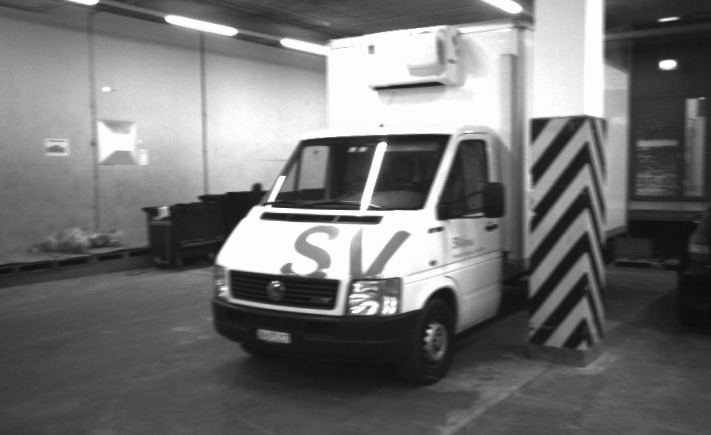
\includegraphics[width=0.16\textwidth]{imgs/ETH3D/rgb/3.jpg} & 
        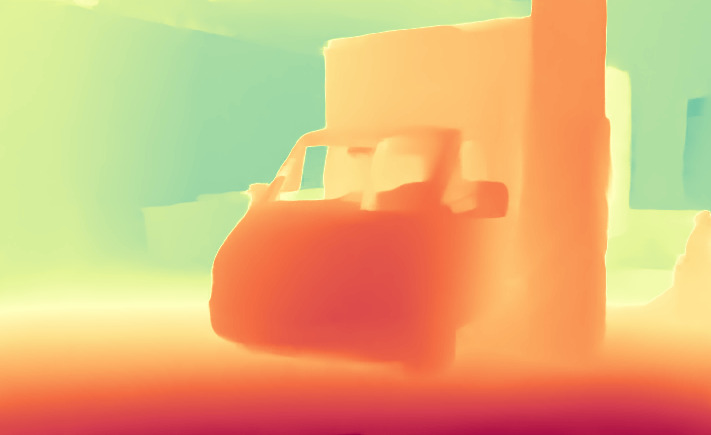
\includegraphics[width=0.16\textwidth]{imgs/ETH3D/stereo/RAFT-Stereo/3.jpg} &
        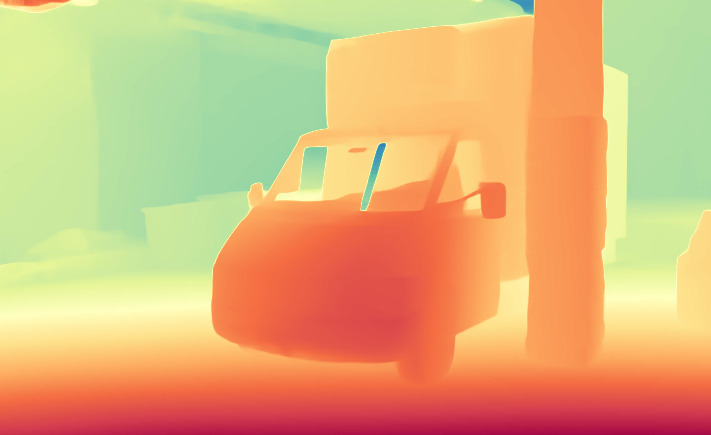
\includegraphics[width=0.16\textwidth]{imgs/ETH3D/stereo/DLNR/3.jpg} &
        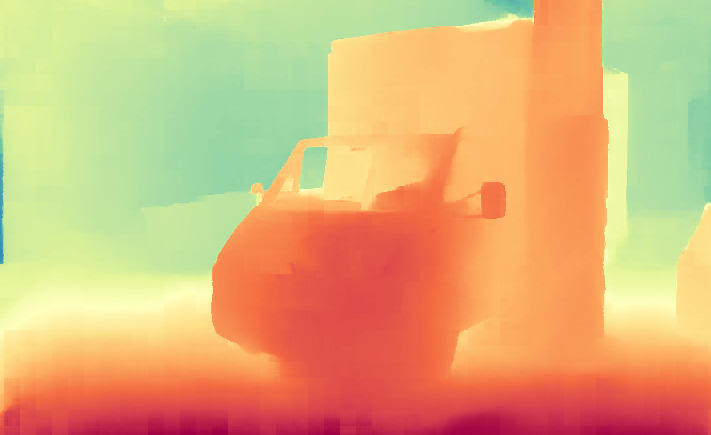
\includegraphics[width=0.16\textwidth]{imgs/ETH3D/stereo/NMRF/3.jpg} &
        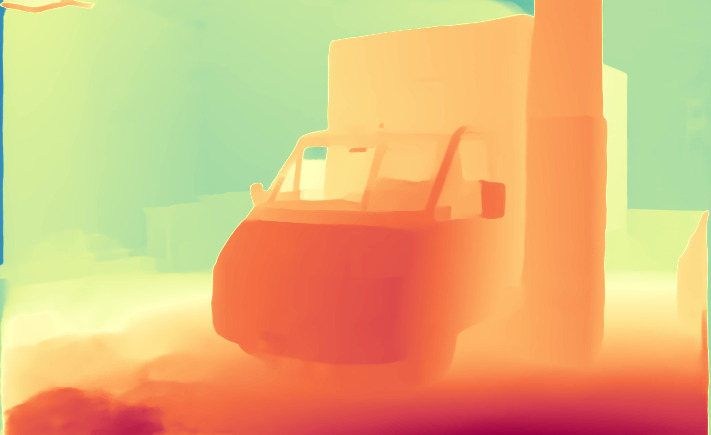
\includegraphics[width=0.16\textwidth]{imgs/ETH3D/stereo/Selective/3.jpg} &
        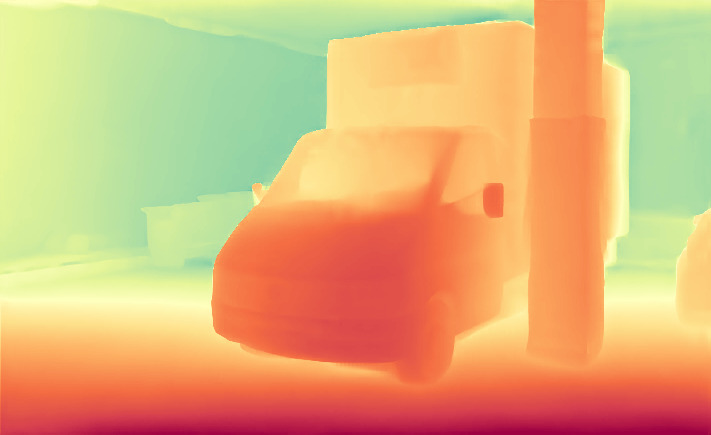
\includegraphics[width=0.16\textwidth]{imgs/ETH3D/stereo/Ours/3.jpg} \\        
    \end{tabular}\vspace{-0.2cm}
    \caption{\textbf{Qualitative Results -- Zero-Shot Generalization.} Predictions by state-of-the-art models and \method.}
    \label{fig:qual_zeroshot}\vspace{-0.3cm}
\end{figure*}

\section{Experiments}
\label{sec:experiments}

We describe our implementation details, datasets, and evaluation protocols, followed by experiments. We also refer the reader to the \textbf{supplementary material} for more results.

\subsection{Implementation and Experimental Settings}

We implement \method using PyTorch, starting from RAFT-Stereo codebase \cite{lipson2021raft}.
We use Depth Anything v2 \cite{depth_anything_v2} as the VFM fueling our model, using the \textit{Large} weights provided by the authors, trained on ground-truth labels from the HyperSim synthetic dataset \cite{roberts2021} only. 

Starting from the Sceneflow RAFT-Stereo checkpoint, we train \method on a single A100 GPU for 3 epochs, with learning rate 1e-4 and AdamW optimizer, on batches of 2 images. We extract random crops of size 320$\times$640 from images and apply standard color and spatial augmentations \cite{lipson2021raft}. 
The VMF is used only to source monocular depth maps, remaining frozen during training.

The number of iterations for GRUs is fixed to 12 during training and increased to 32 at inference time.

\subsection{Evaluation Datasets \& Protocol}

\textbf{Datasets}. We utilize SceneFlow \cite{mayer2016large} as our sole training dataset, comprising about 39k synthetic stereo pairs with dense ground-truth disparities. For evaluation, we employ several benchmarks: Middlebury 2014 \cite{scharstein2014high} and its 2021 extension \cite{middlebury2021} provide high-resolution indoor scenes with semi-dense labels (15 and 24 stereo pairs), KITTI 2012 \cite{geiger2012we} and 2015 \cite{menze2015object} feature outdoor driving scenarios ($\sim$200 pairs each at $1280 \times 384$ with sparse LiDAR ground truth), and ETH3D \cite{schops2017multi} contributes 27 low-resolution indoor/outdoor scenes. For non-Lambertian surfaces, we primarily use Booster \cite{zamaramirez2022booster}, containing 228 high-resolution (12 Mpx) indoor pairs with its 191-pair online benchmark, and LayeredFlow \cite{wen2024layeredflow}, featuring 400 pairs with transparent objects and sparse ground truth ($\sim$50 points per pair). Additionally, we include our newly proposed MonoTrap dataset focusing on optical illusions. For zero-shot evaluation, we test on KITTI 2015, Middlebury v3 at half (H) resolution, Middlebury 2021, and ETH3D, while non-Lambertian zero-shot testing relies on Booster at quarter (Q) resolution and LayeredFlow at eight (E) resolution.

\textbf{Evaluation Metrics}. We evaluate our method using two standard metrics: the average pixel error (Avg.), which computes the absolute difference between predicted and ground truth disparities averaged over all pixels, and the bad$>\tau$ error, which measures the percentage of pixels with a disparity error greater than $\tau$ pixels -- for the latter, we compute it considering all pixels or either non-occluded or occluded pixels, referred to as \textit{All}, \textit{Noc} or \textit{Occ} respectively. 

We evaluate on \dataset through standard monocular depth metrics \cite{godard2017unsupervised} - Absolute relative error (AbsRel), RMSE, and $\delta<1.05$ score.


\begin{table*}
\centering
\renewcommand{\tabcolsep}{14pt}
\scalebox{0.78}{
\begin{tabular}{|l||rrrrr|rrrr|}
\multicolumn{1}{c}{} & \multicolumn{5}{c}{Booster (Q)} & \multicolumn{4}{c}{LayeredFlow (E)} \\
\hline
 \multirow{2}{*}{Model} & \multicolumn{4}{c}{Error Rate (\%)} & Avg. & \multicolumn{3}{c}{Error Rate (\%)} & Avg. \\
  & $>2$ & $>4$ & $>6$ & $>8$ & (px) & $>1$ & $>3$ & $>5$ &(px) \\
\hline\hline
{RAFT-Stereo} \cite{lipson2021raft}
& \snd 17.84 & \snd 13.06 & \snd 10.76 & \snd 9.24 & \snd 3.59
& \trd 89.21 & \snd 79.02 & 71.61 & \trd 19.27 \\
{PSMNet} \cite{chang2018pyramid}
& 34.47 & 24.83 & 20.46 & 17.77 & 7.26
& 91.85 & 79.84 & \snd 70.04 & 21.18 \\
{GMStereo} \cite{xu2023unifying}
& 32.44 & 22.52 & 17.96 & 15.02 & 5.29
& 92.95 & 83.68 & 74.76 & 20.91 \\
{ELFNet} \cite{lou2023elfnet}
& 45.52 & 35.79 & 30.72 & 27.33 & 14.04
& 93.08 & 82.24 & \trd 70.41 & 20.19 \\
{PCVNet} \cite{Zeng_2023_ICCV}
& 31.08 & 22.90 & 18.80 & 16.15 & 6.16
& 91.64 & 80.75 & 74.34 & 20.85 \\
{DLNR} \cite{zhao2023high}
& 18.56 & 14.55 & 12.61 & 11.22 & \trd 3.97
& 89.90 & 79.46 & 72.72 & \snd 18.97 \\
{Selective-RAFT} \cite{wang2024selective}
& 20.01 & 15.08 & 12.52 & 10.88 & 4.12
& 92.69 & 86.32 & 78.82 & 20.18 \\
{Selective-IGEV} \cite{wang2024selective}
& \trd 18.52 & \trd 14.24 & \trd 12.14 & \trd 10.77 & 4.38
& 91.31 & 81.72 & 74.74 & 19.65 \\
{IGEV-Stereo} \cite{xu2023iterative}
& 23.38 & 14.45 & 12.61 & 11.41 & 4.91
& 92.54 & 81.42 & 74.74 & 20.88 \\
{NMRF} \cite{guan2024neural}
& 27.08 & 19.06 & 15.43 & 13.21 & 5.02
& \snd 89.08 & \trd 79.13 & 70.51 & 20.17 \\
{\bf \method{} (ours)}
&\fst 9.96 &\fst 5.81 &\fst 4.48 &\fst 3.79 &\fst 1.36
&\fst 80.83 &\fst 58.21 &\fst 46.48 &\fst 12.14 \\

\hline

\end{tabular}}\vspace{-0.2cm}
\caption{\textbf{Zero-shot Non-Lambertian Generalization.} Comparison with state-of-the-art models. Networks trained on SceneFlow \cite{mayer2016large}.
}\vspace{-0.3cm}
\label{tab:roundtable2}
\end{table*}

\begin{figure*}[t]
    \centering
    \renewcommand{\tabcolsep}{1pt}
    \begin{tabular}{ccccccc}
        & \small RGB &
        \small RAFT-Stereo \cite{lipson2021raft} &
        \small DLNR \cite{zhao2023high} &
        \small NMRF \cite{guan2024neural} &
        \small Selective-IGEV \cite{wang2024selective} &
        \method \\
        
        \hspace{-3.5em}\rotatebox[origin=c]{90}{\raisebox{0.08\textwidth}{\parbox[c][0.10\textwidth][c]{0.10\textwidth}{\centering\small Booster}}}\hspace{-3.5em} &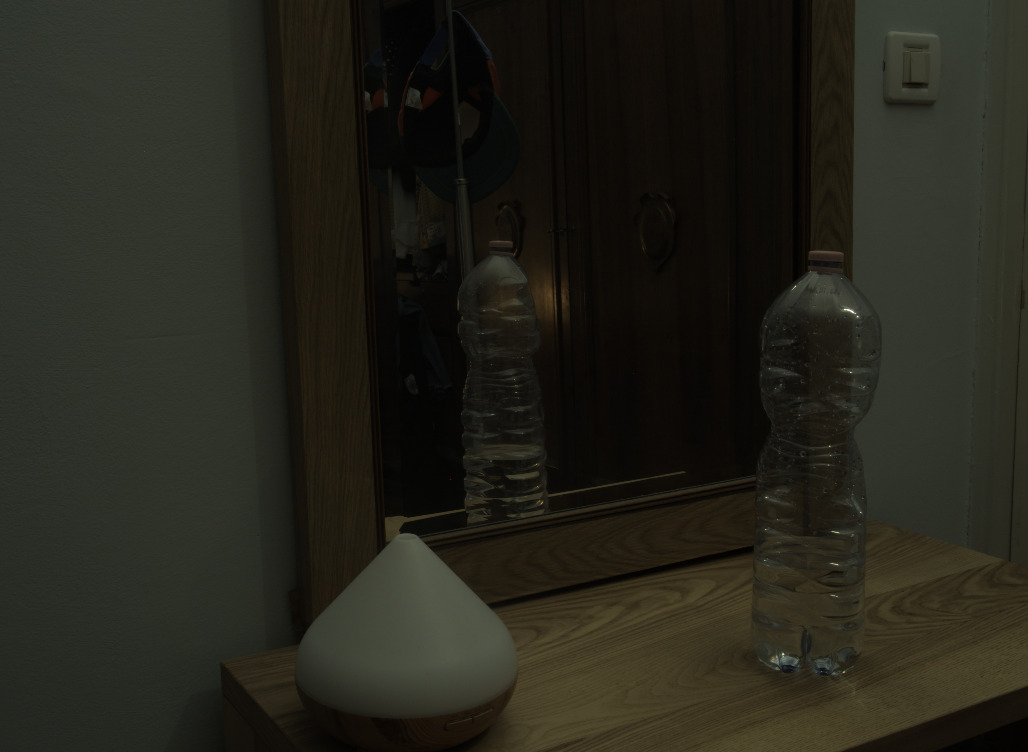
\includegraphics[width=0.16\textwidth]{imgs/booster/rgb/19.jpg} & 
        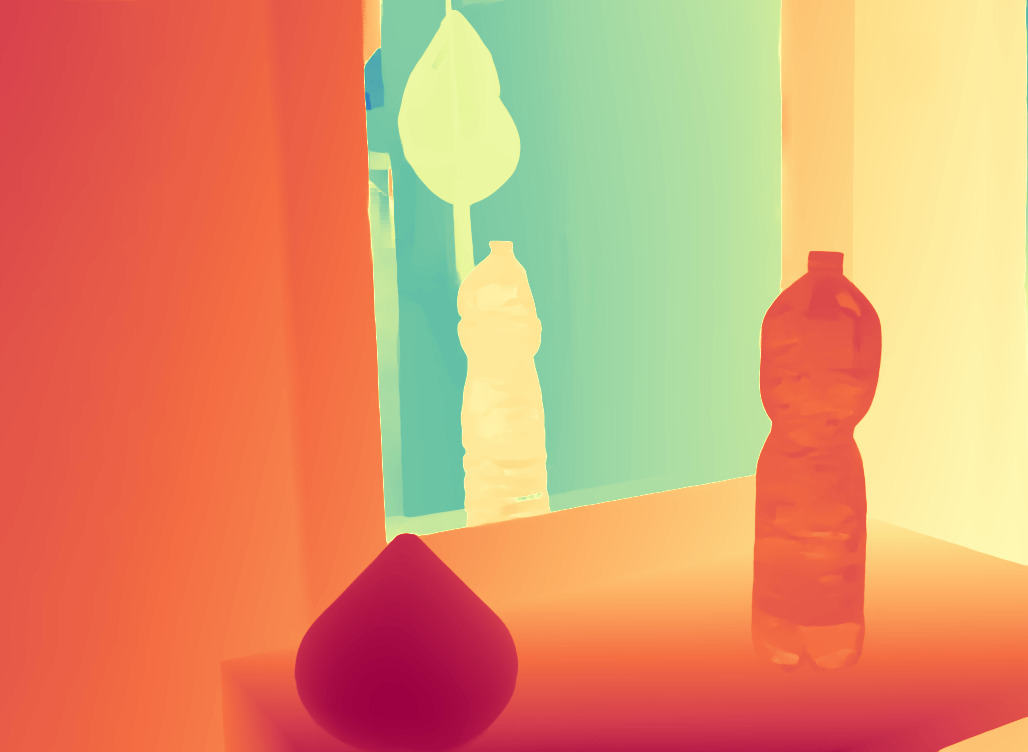
\includegraphics[width=0.16\textwidth]{imgs/booster/stereo/RAFT-Stereo/19.jpg} &
        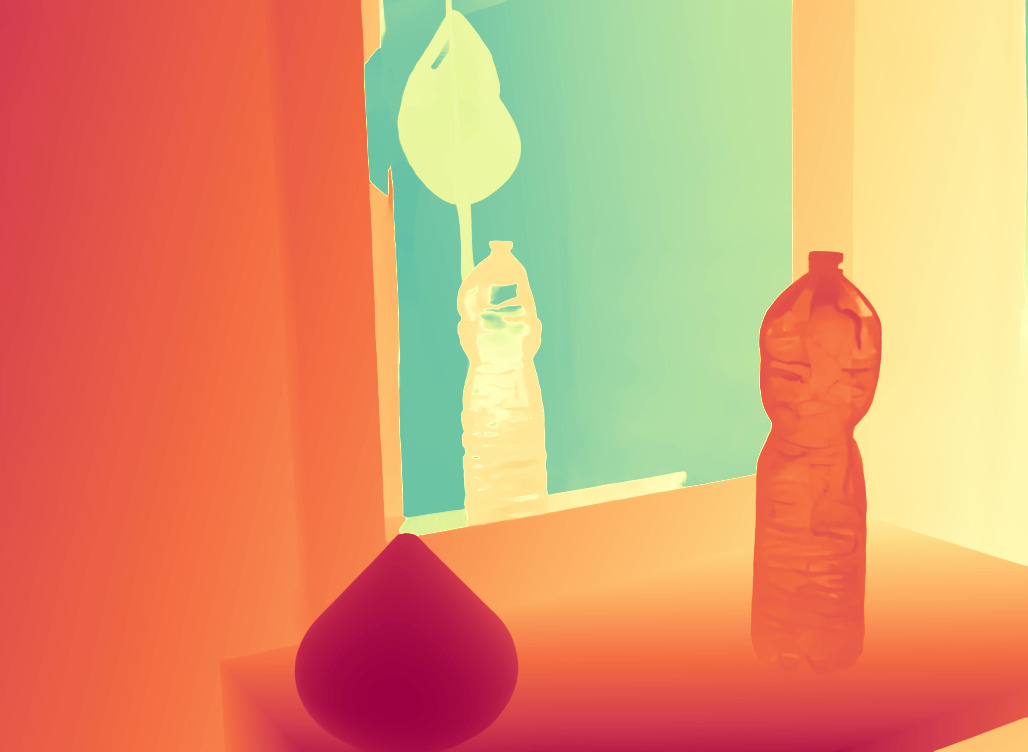
\includegraphics[width=0.16\textwidth]{imgs/booster/stereo/DLNR/19.jpg} &
        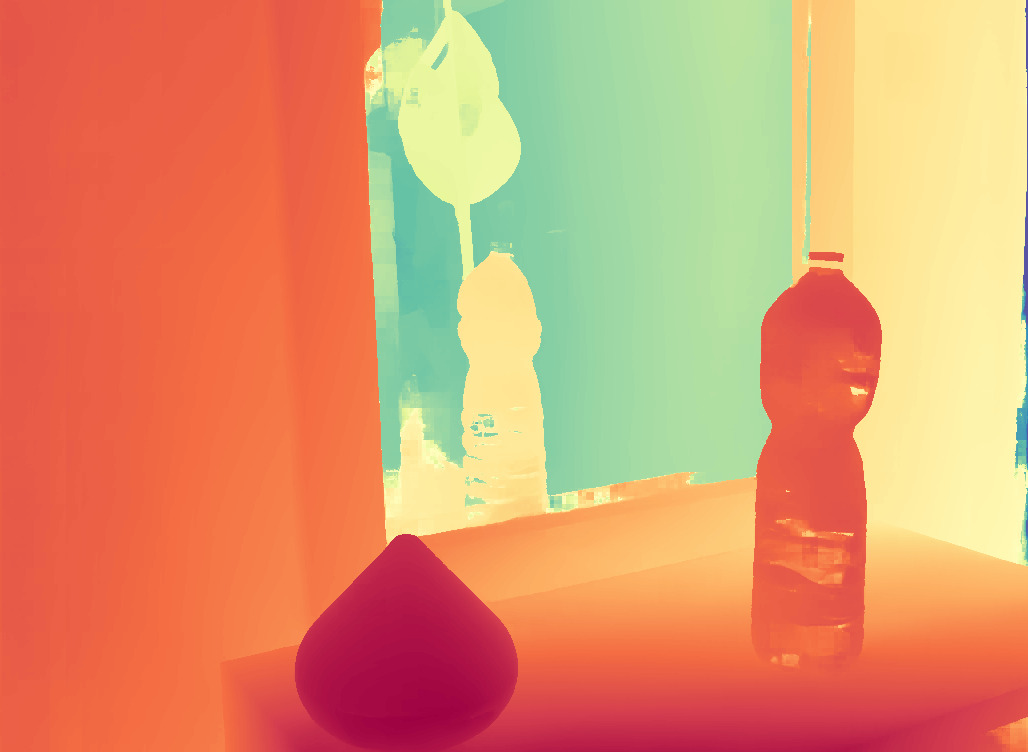
\includegraphics[width=0.16\textwidth]{imgs/booster/stereo/NMRF/19.jpg} &
        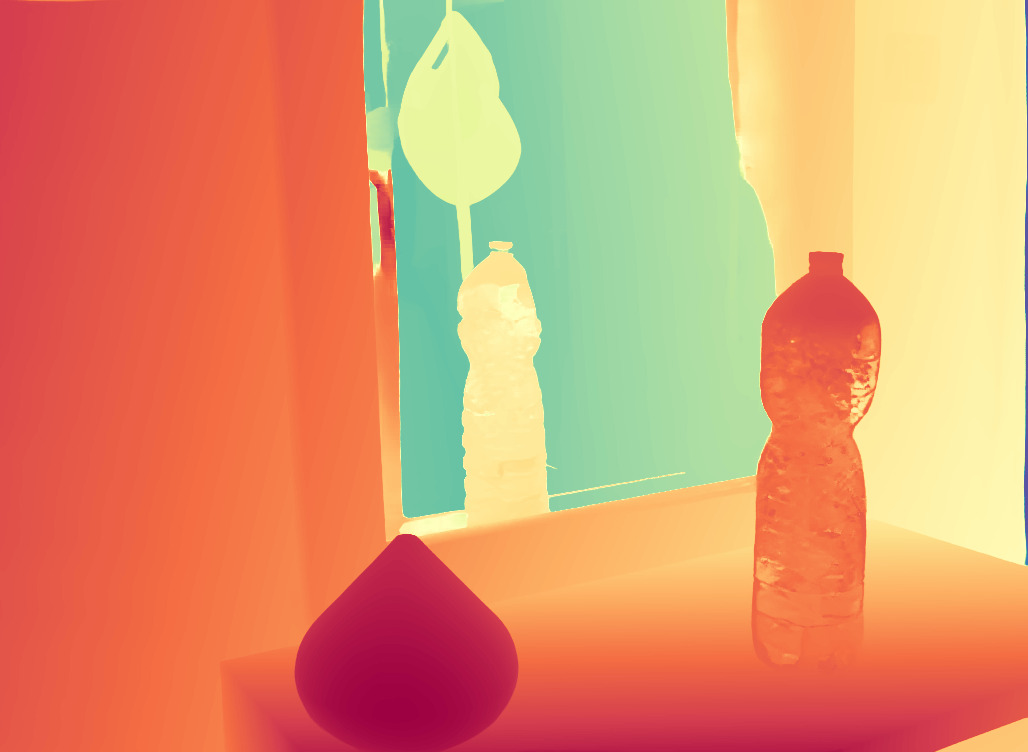
\includegraphics[width=0.16\textwidth]{imgs/booster/stereo/Selective/19.jpg} &
        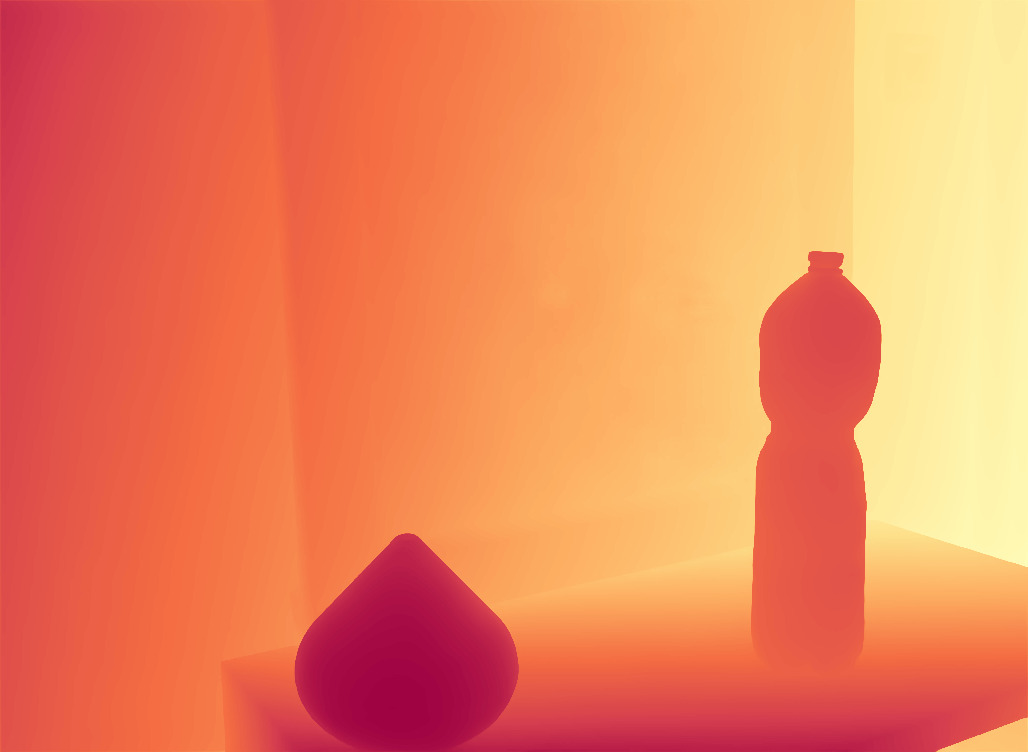
\includegraphics[width=0.16\textwidth]{imgs/booster/stereo/Ours/19.jpg} \vspace{-0.5cm}\\


        \hspace{-3.5em}\rotatebox[origin=c]{90}{\raisebox{0.08\textwidth}{\parbox[c][0.10\textwidth][c]{0.10\textwidth}{\hspace{-0.3cm}\small LayeredFlow}}}\hspace{-3.5em} &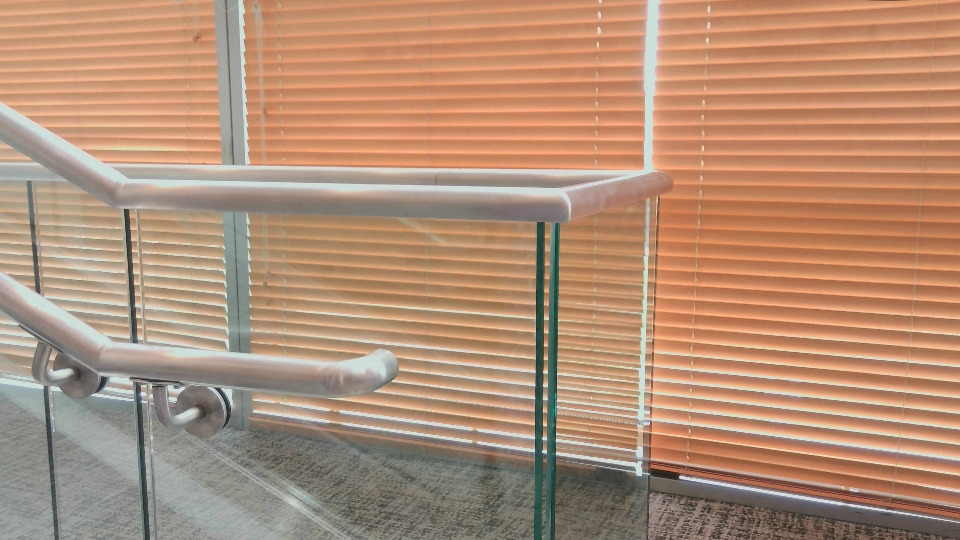
\includegraphics[width=0.16\textwidth]{imgs/Layered/left.jpg} & 
        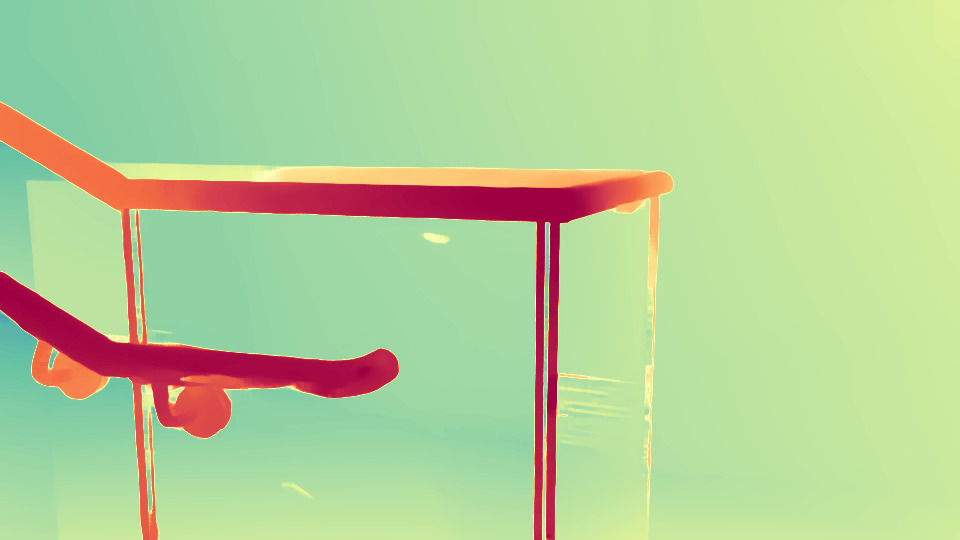
\includegraphics[width=0.16\textwidth]{imgs/Layered/raftstereo.jpg} &
        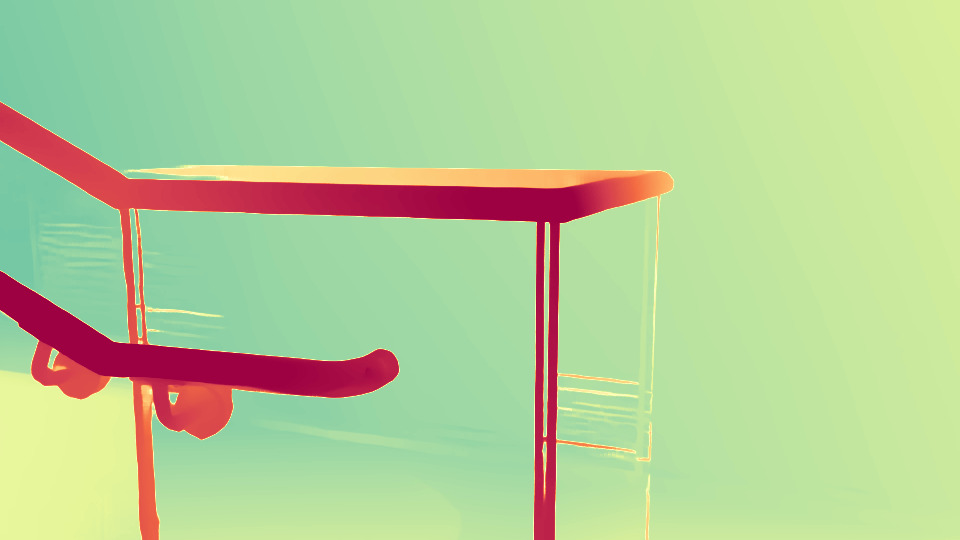
\includegraphics[width=0.16\textwidth]{imgs/Layered/dlnr.jpg} &
        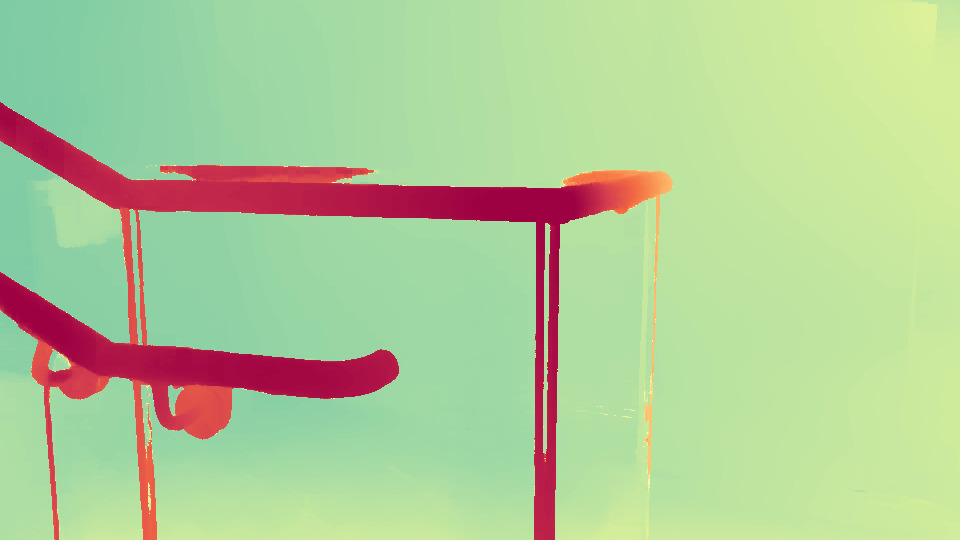
\includegraphics[width=0.16\textwidth]{imgs/Layered/nmrf.jpg} &
        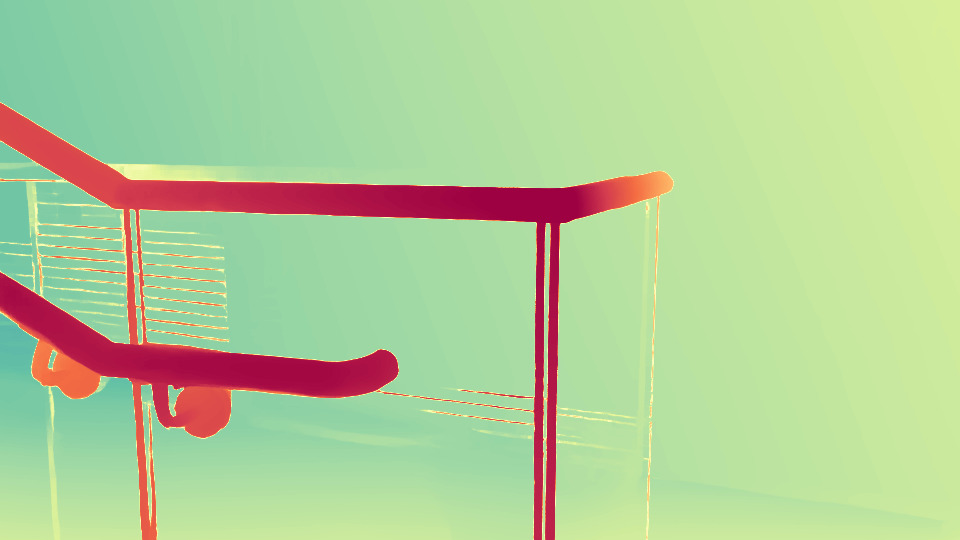
\includegraphics[width=0.16\textwidth]{imgs/Layered/selectiveigev.jpg} &
        
\includegraphics[width=0.16\textwidth]{imgs/Layered/ours.jpg} \\
        
    \end{tabular}\vspace{-0.2cm}
    \caption{\textbf{Qualitative results -- Zero-Shot non-Lambertian Generalization.} Predictions by state-of-the-art models and \method.}
    \label{fig:qual_nonlambertian}\vspace{-0.3cm}
\end{figure*}

\subsection{Ablation Study}

We start our analysis by evaluating how individual components of our model contribute to the overall accuracy. All model variants are trained solely on the synthetic SceneFlow dataset and tested on Booster and Middlebury 2014, allowing us to examine their effectiveness on non-Lambertian surfaces and general scenes. 

Table \ref{tab:ablation} summarizes our findings. In (A), we report the performance of our baseline model, upon which we build \method -- i.e., RAFT-stereo \cite{lipson2021raft}. On the one hand, by adding monocular context from an off-the-shelf monocular depth network to the pre-trained context backbone (B), we observe improved performance on non-Lambertian surfaces, though at the expense of a general drop in accuracy on Middlebury. On the other hand, by re-training the context backbone to process depth maps obtained from the monocular network on SceneFlow (C), we can appreciate a consistent improvement in both datasets. 
Introducing the normals correlation volume with subsequent differentiable depth scaling (D) significantly enhances the accuracy on non-Lambertian surfaces, also showing improvements on indoor scenes.
Finally, cost volume augmentations and truncation (E) demonstrate positive effects on transparent surfaces and mirrors present in the Booster dataset by further reducing the bad-2 metric by approximately 1.5\% and Avg. by 0.5 pixels, with minimal influence on Middlebury.

According to these results, from now on, we will adopt (E) as the default setting for \method.

\subsection{Zero-Shot Generalization}

We now compare our \method model against state-of-the-art deep stereo networks, assessing zero-shot generalization capability when transferred from synthetic to real images.
Purposely, we follow a well-established benchmark in the literature \cite{lipson2021raft,Tosi_2023_CVPR}, evaluating on real datasets models pre-trained exclusively on SceneFlow \cite{mayer2016large}.

Table \ref{tab:roundtable1} compares \method with off-the-shelf stereo networks using authors' provided weights. Considering All, Noc, and Avg. metrics, we can notice how \method achieves consistently better results across most datasets, achieving almost 3\% lower bad-2 All on Middlebury 2014 versus the second-best method DLNR \cite{zhao2023high}, and breaking the 4\% barrier on KITTI's bad-3 All metric. 

The Occ metric further demonstrates how \method{} consistently outperforms other stereo models on any dataset, with substantial margins over the second-best -- i.e., approximately 7\% on Middlebury 2014 and KITTI 2012, and 3\% on ETH3D. This confirms that leveraging priors from VFMs for monocular depth estimation effectively improve the stereo matching estimation accuracy in challenging conditions where stereo matching is ill-posed, such as at occluded regions.

Figure \ref{fig:qual_zeroshot} shows predictions on KITTI 2015, Middlebury 2014, and ETH3D samples. In particular, the first row shows an extremely challenging case for SceneFlow-trained models, where \method achieves accurate disparity maps thanks to VFM priors. 



\subsection{Zero-Shot Non-Lambertian Generalization}

We now assess the generalization capabilities of \method and existing stereo models when dealing with non-Lambertian materials, such as transparent surfaces or mirrors. To this end, we conduct a zero-shot generalization evaluation experiment on the Booster \cite{Ramirez_2022_CVPR} and LayeredFlow \cite{wen2024layeredflow} datasets, once again using models pre-trained on SceneFlow \cite{mayer2016large} -- with weights provided by the authors. 

Table \ref{tab:roundtable2} shows the outcome of this evaluation. This time, we can perceive even more clearly how \method is the absolute winner, demonstrating unprecedented robustness in the presence of non-Lambertian surfaces despite being trained only on synthetic stereo data, not even featuring such objects. These results further validate how leveraging strong priors from existing VFMs for monocular depth estimation can play a game-changing role in stereo matching as well, especially when lacking training data explicitly targeting critical conditions such as non-Lambertian surfaces.

Figure \ref{fig:qual_nonlambertian} shows examples from Booster and LayeredFlow, where \method is the only stereo model correctly perceiving the mirror and transparent railing.


\begin{table}[t]
\centering
\renewcommand{\tabcolsep}{10pt}
\scalebox{0.76}{
\begin{tabular}{|l||rrr|}
\multicolumn{1}{c}{} & \multicolumn{3}{c}{\dataset} \\
\hline
 \multirow{2}{*}{Model} & AbsRel & RMSE & $\sigma<1.05$ \\
  & (\%)$\downarrow$ & (m)$\downarrow$ & (\%)$\uparrow$ \\
\hline\hline
Depth Anything v2 \cite{depth_anything_v2} & 35.00 & 0.34 & 27.62 \\
Depth Anything v2 \cite{depth_anything_v2} $\dagger$ & 21.81 & 0.28 & 29.31 \\
DepthPro \cite{depthpro} & 29.96 & 0.30 & 27.81 \\
DepthPro \cite{depthpro} $\dagger$ & \trd 17.23 & \trd 0.25 & \trd 37.85 \\
\hline
RAFT-Stereo \cite{lipson2021raft} & \snd 4.62 & \snd 0.12 & \snd 75.15 \\
\textbf{\method} & \fst 4.59 & \fst 0.11 & \fst 77.26 \\

\hline

\end{tabular}}\vspace{-0.2cm}
\caption{\textbf{\dataset Benchmark.} Comparison with state-of-the-art monocular depth estimation models and RAFT-Stereo. Both RAFT-Stereo and \method are trained on SceneFlow \cite{mayer2016large}. $\dagger$ refers to robust scaling through RANSAC.
}\vspace{-0.3cm}
\label{tab:monotrap}
\end{table}




\subsection{\dataset Benchmark}

We conclude our evaluation by running experiments on our newly collected \dataset dataset to prove the robustness of \method in the presence of critical conditions harming the accuracy of monocular depth predictors.

Table \ref{tab:monotrap} collects the results achieved by state-of-the-art monocular depth estimation models, the baseline stereo model over which we built our framework (RAFT-Stereo) and \method. Regarding the former models, as they predict affine-invariant depth maps, following the literature \cite{Ranftl2022} we use least square errors to align them to the ground-truth. As these models are fooled by the visual illusions, this scaling procedure is likely to yield sub-optimal scale and shift parameters. Therefore, we alternatively align to ground-truth depth through a more robust RANSAC fitting -- denoted with $\dagger$ in the table.

On the one hand, by comparing monocular and stereo methods, we notice how the failures of the former negatively impact their evaluation metrics. Once again, we remark that a direct comparison across the two families of methods is not the main goal of this experiment.
On the other hand, we focus on the comparison between RAFT-Stereo and \method, with our model performing slightly better than its baseline. This fact proves that despite its strong reliance on the priors retrieved from VFMs for monocular depth estimation, \method can properly ignore such priors when unreliable. 

Figure \ref{fig:qual_monotrap} shows three samples where Depth Anything v2 fails while \method does not.

\begin{figure}[t]
    \centering
    \renewcommand{\tabcolsep}{1pt}
    \begin{tabular}{ccc}
        \small RGB &
        \small D. Anything v2 \cite{depth_anything_v2} &
        \method \\
        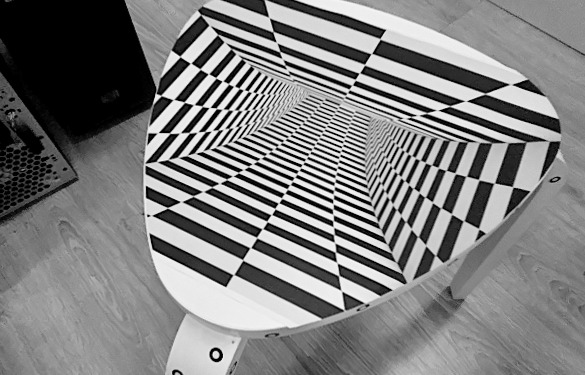
\includegraphics[width=0.16\textwidth]{imgs/monotrap_samples/rgb/13.jpg} & 
        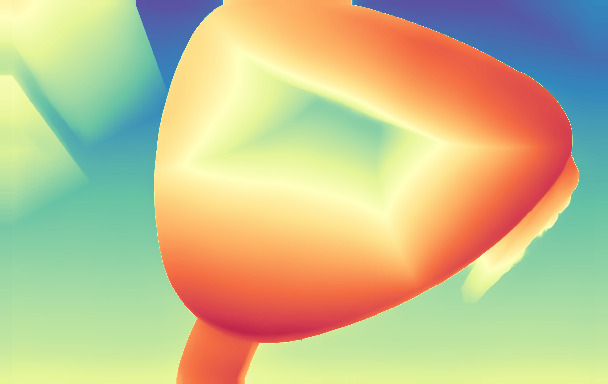
\includegraphics[width=0.16\textwidth]{imgs/monotrap_samples/mono/13.jpg} &
        
\includegraphics[width=0.16\textwidth]{imgs/monotrap_samples/Ours/13.jpg} \\

        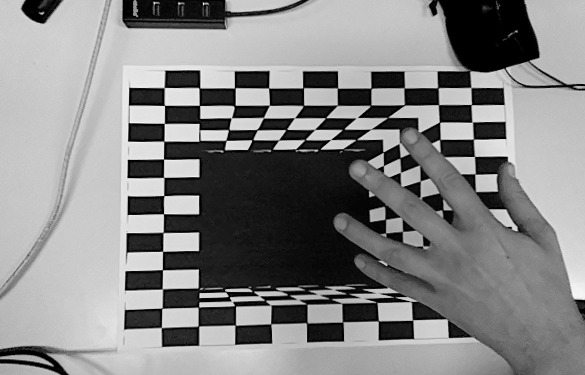
\includegraphics[width=0.16\textwidth]{imgs/monotrap_samples/rgb/2.jpg} & 
        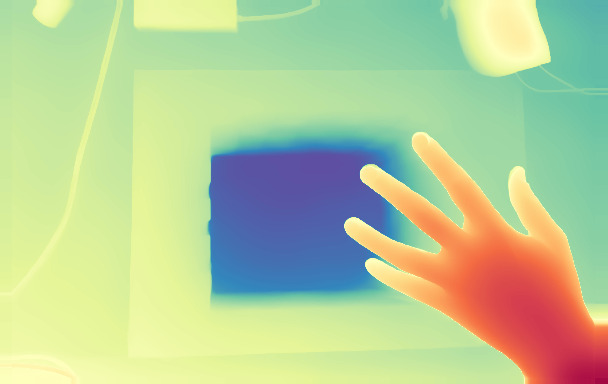
\includegraphics[width=0.16\textwidth]{imgs/monotrap_samples/mono/2.jpg} &
        
\includegraphics[width=0.16\textwidth]{imgs/monotrap_samples/Ours/2.jpg} \\

        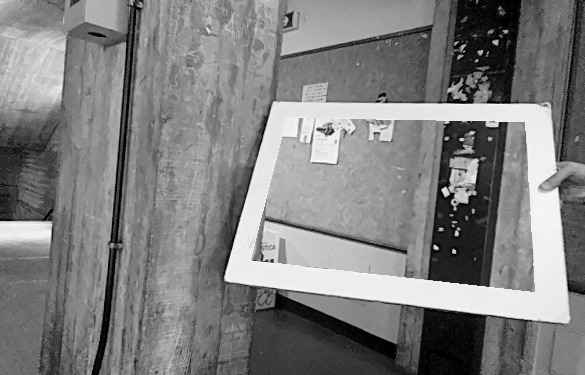
\includegraphics[width=0.16\textwidth]{imgs/monotrap_samples/rgb/30.jpg} & 
        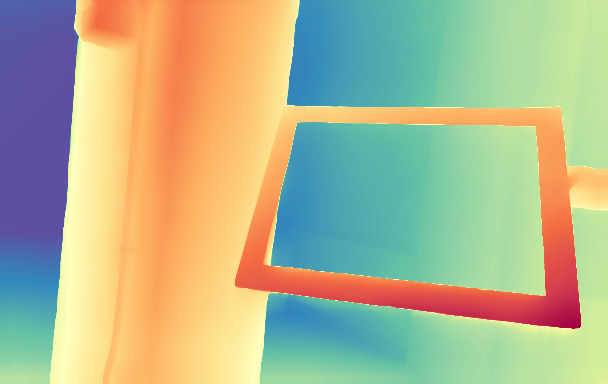
\includegraphics[width=0.16\textwidth]{imgs/monotrap_samples/mono/30.jpg} &
        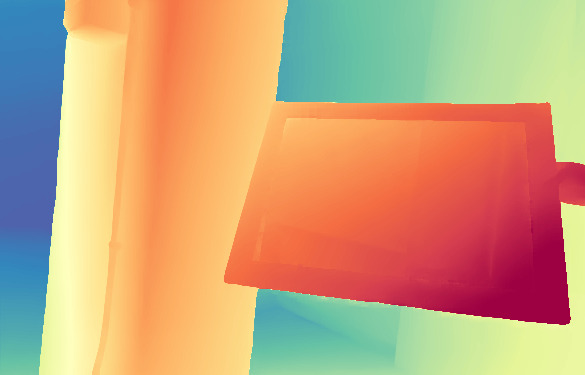
\includegraphics[width=0.16\textwidth]{imgs/monotrap_samples/Ours/30.jpg} \\

        
    \end{tabular}\vspace{-0.2cm}
    \caption{\textbf{Qualitative results -- \dataset.} \method is not fooled by erroneous predictions by its monocular engine \cite{depth_anything_v2}. }
    \label{fig:qual_monotrap}\vspace{-0.3cm}
\end{figure}
